\documentclass[xcolor=pdftex,dvipsnames,table,mathserif]{beamer}
%\usepackage{subfigure}
\usepackage{amsbsy}
\usepackage{tikz}
\usetikzlibrary{arrows}
\usepackage{amsmath,graphicx,dsfont,color}
\usepackage{amsfonts}
\usepackage{amssymb}
\usepackage{array}

\usepackage{subfig}

% makes the subfig package work
\makeatletter
\let\@@magyar@captionfix\relax
\makeatother

% subfigure counter resets every frame
\makeatletter
\@addtoreset{subfigure}{framenumber}
\makeatother

% First author and year
\bibliographystyle{apalike}

% This sets the list items of the bibliography to the same symbol used for citation.
\setbeamertemplate{bibliography item}{\insertbiblabel}

% This avoids extralines for different entries
\setbeamertemplate{bibliography entry title}{}
\setbeamertemplate{bibliography entry location}{}
\setbeamertemplate{bibliography entry note}{}

\DeclareMathOperator*{\argmin}{arg\,min}
\DeclareMathOperator*{\argmax}{arg\,max}
%Definitiona

\newcommand{\x}{\mathbf{x}}
\newcommand{\X}{\mathbf{X}}
\newcommand{\W}{\mathbf{W}} %Weight
\newcommand{\bais}{\mathbf{b}}%Bais
\newcommand{\act}{\texttt{g}}%Activation
\newcommand{\loss}{L}
\newcommand{\pdata}{\hat{p}_{\texttt{data}}}
\newcommand{\nsize}{N}
\newcommand{\nfeatures}{P}
\newcommand{\param}{\boldsymbol{\theta}}
\newcommand{\featmap}{\boldsymbol{\phi}}
\newcommand{\EV}{\mathbb{E}}







\usepackage{physics}

\AtBeginSection[]{
  \begin{frame}{Contents}
  \tableofcontents[currentsection, hideothersubsections]
  \end{frame}
}

\AtBeginSubsection[]{
  \begin{frame}{Contents}
  \tableofcontents[currentsection, subsectionstyle=show/shaded/hide]
  \end{frame}
}

\setbeamertemplate{footline}[frame number]{}
\setbeamertemplate{navigation symbols}{}
\setbeamertemplate{section in toc}[square]
\setbeamertemplate{items}[square]

\title{Artificial neural networks and backpropagation}
\author{E. Decencière}
\date{MINES ParisTech\\
  PSL Research University\\
  Center for Mathematical Morphology
}
\titlegraphic{
\includegraphics[height=1.7cm]{../graphics/logoemp}}

\useinnertheme{rounded}
\usecolortheme{rose}

%%%%%%%%%%%%%%%%%%%%%%%%%%%%%%%%%%%%%%%%%%%%%%%%%%
%%%%%%%%%%%%%%%%%%%%%%%%%%%%%%%%%%%%%%%%%%%%%%%%%%
\begin{document}
\begin{frame}
\titlepage
\end{frame}

\frame{
\frametitle{Contents}
\tableofcontents[hidesubsections]
}


%%%%%%%%%%%%%%%%%%%%%%%%%%%%%%%%%%%%%%%%%%%%%%%%%%
\section{Introduction}
%%%%%%%%%%%%%%%%%%%%%%%%%%%%%%%%%%%%%%%%%%%%%%%%%%

\frame{
\frametitle{Artificial neural networks and deep learning history}


\begin{block}{}
  For a very complete state of the art on deep learning, see the overview by Schmidhuber \cite{schmidhuber_deep_2015}.
\end{block}

\begin{itemize}
\item 1958: Rosenblatt's perceptron \cite{rosenblatt_perceptron:_1958}
\item 1980's: the backpropagation algorithm (see, for example, the work of Le Cun \cite{lecun_procedure_1985})
\item 2006-: CNN implementations using Graphical Processing Units (GPU): up to a 50 speed-up factor.
\item 2011-: super-human performances \cite{ciresan_committee_2011}
\item 2012: Imagenet image classification won by a CNN \cite{krizhevsky_imagenet_2012}.

\end{itemize}

}

%%%%%%%%%%%%%%%%%%%%%%%%%%%%%%%%%%%%%%%%%%%%%%%%%%
\section{Artificial neuron}
%%%%%%%%%%%%%%%%%%%%%%%%%%%%%%%%%%%%%%%%%%%%%%%%%%

\frame{
\frametitle{Neuron}

\begin{figure}
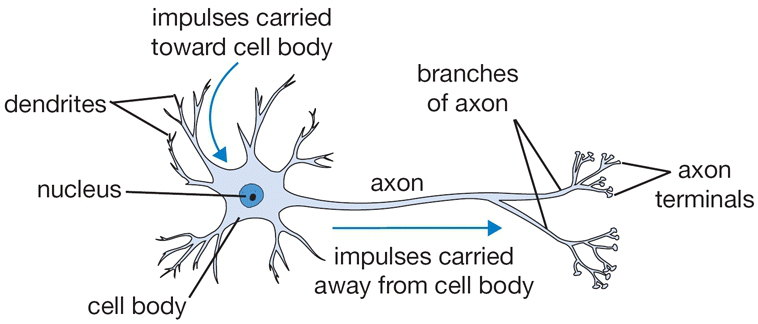
\includegraphics[height=3cm]{../graphics/neuron}
\end{figure}

\begin{itemize}
\item The human brain contains 100 billion ($10^{11}$) neurons
\item A human neuron can have several thousand dendrites
\item The neuron sends a signal through its axon if during a given interval of time the net input signal (sum on excitatory and inhibitory signals received through its dentrites) is larger than a threshold.
\end{itemize}

}

%%%%%%%%%%%%%%%%%%%%%%%%%%%%%%%%%%%%%%%%%%%%%%%%%%

\frame{
\frametitle{Artificial neuron}

\begin{figure}
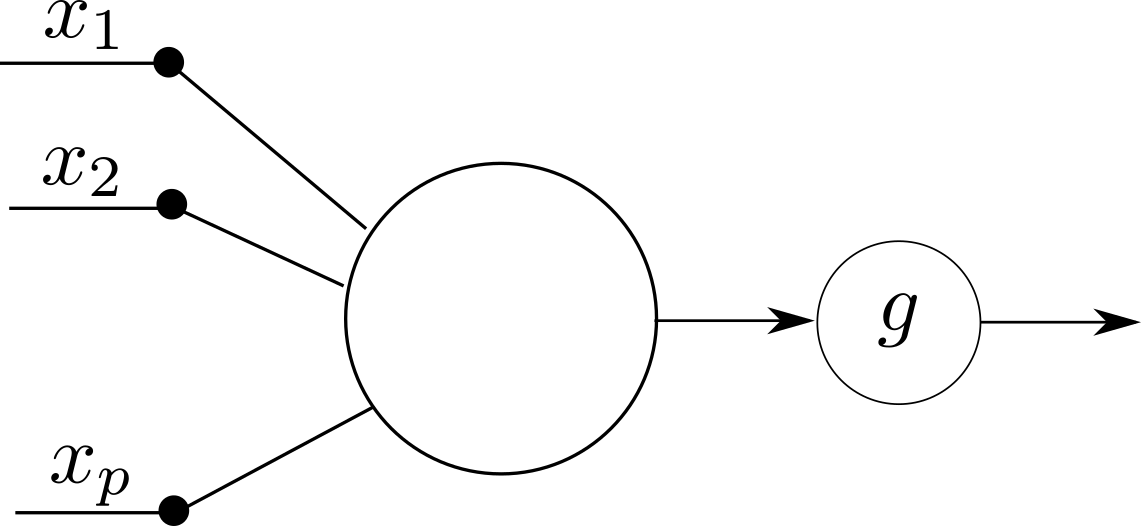
\includegraphics[height=3cm]{../graphics/neurone_general}
\end{figure}

\begin{block}{General principle}
An artificial neuron takes $p$ inputs $\{x_i\}_{1 \leq i \leq p}$, combines them to obtain a single value, and applies an \alert{activation function} $\act$ to the result.
\end{block}

\begin{itemize}
\item The first artificial neuron model was proposed by \cite{mcculloch_logical_1943}
\item Input and output signals were binary
\item Input dendrites could be inhibitory or excitatory
\end{itemize}

}

%%%%%%%%%%%%%%%%%%%%%%%%%%%%%%%%%%%%%%%%%%%%%%%%%%

\frame{
  \frametitle{Modern artificial neuron}

  \begin{figure}
    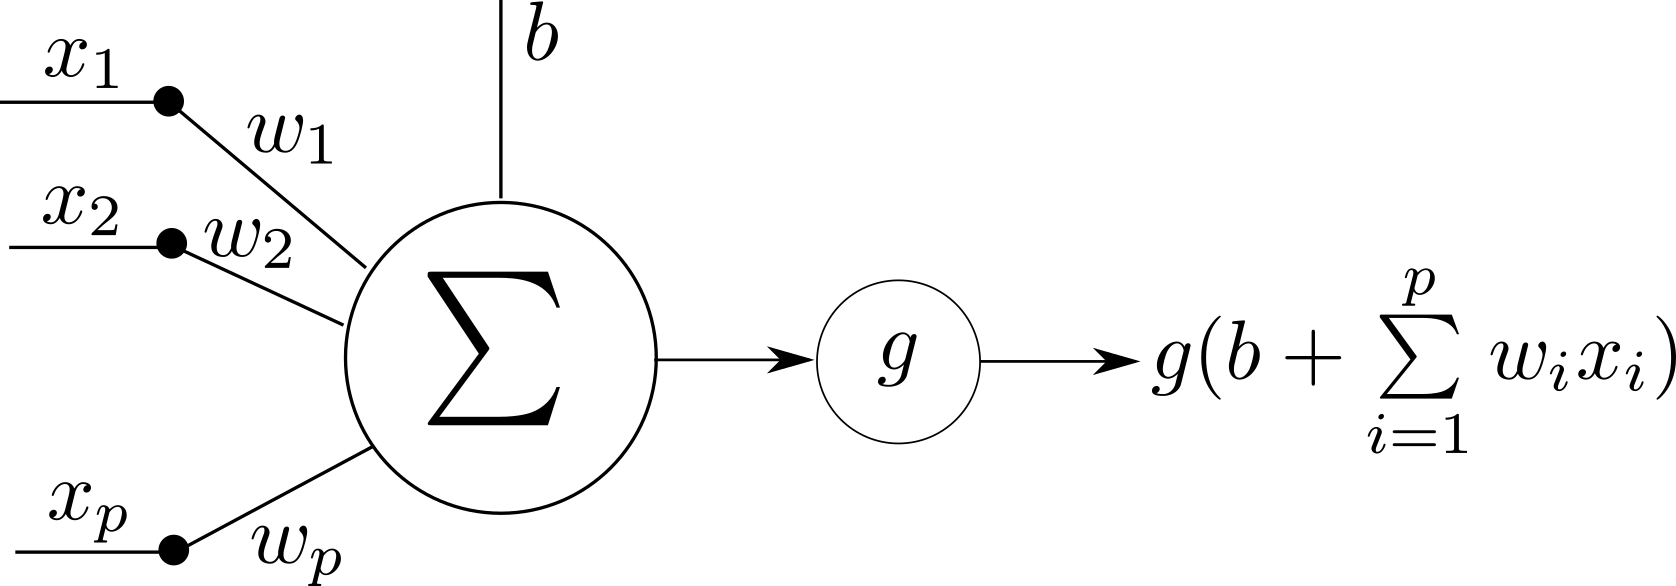
\includegraphics[height=3cm]{../graphics/neurone}
  \end{figure}

  \begin{itemize}
  \item The neuron computes a linear combination of the \alert{inputs} $x_i$
    \begin{itemize}
    \item The \alert{weights} $w_i$ are multiplied with the inputs
    \item The \alert{bias} $b$ can be interpreted as a threshold on the sum
    \end{itemize}

  \item The \alert{activation function} $\act$ somehow decides, depending on its input, if a signal (the neuron's \alert{activation}) is produced
  \end{itemize}


}

%%%%%%%%%%%%%%%%%%%%%%%%%%%%%%%%%%%%%%%%%%%%%%%%%%
\subsection{Activation functions}
%%%%%%%%%%%%%%%%%%%%%%%%%%%%%%%%%%%%%%%%%%%%%%%%%%

%%%%%%%%%%%%%%%%%%%%%%%%%%%%%%%%%%%%%%%%%%%%%%%%%%

\frame{
  \frametitle{The role of the activation function}

  \begin{figure}
    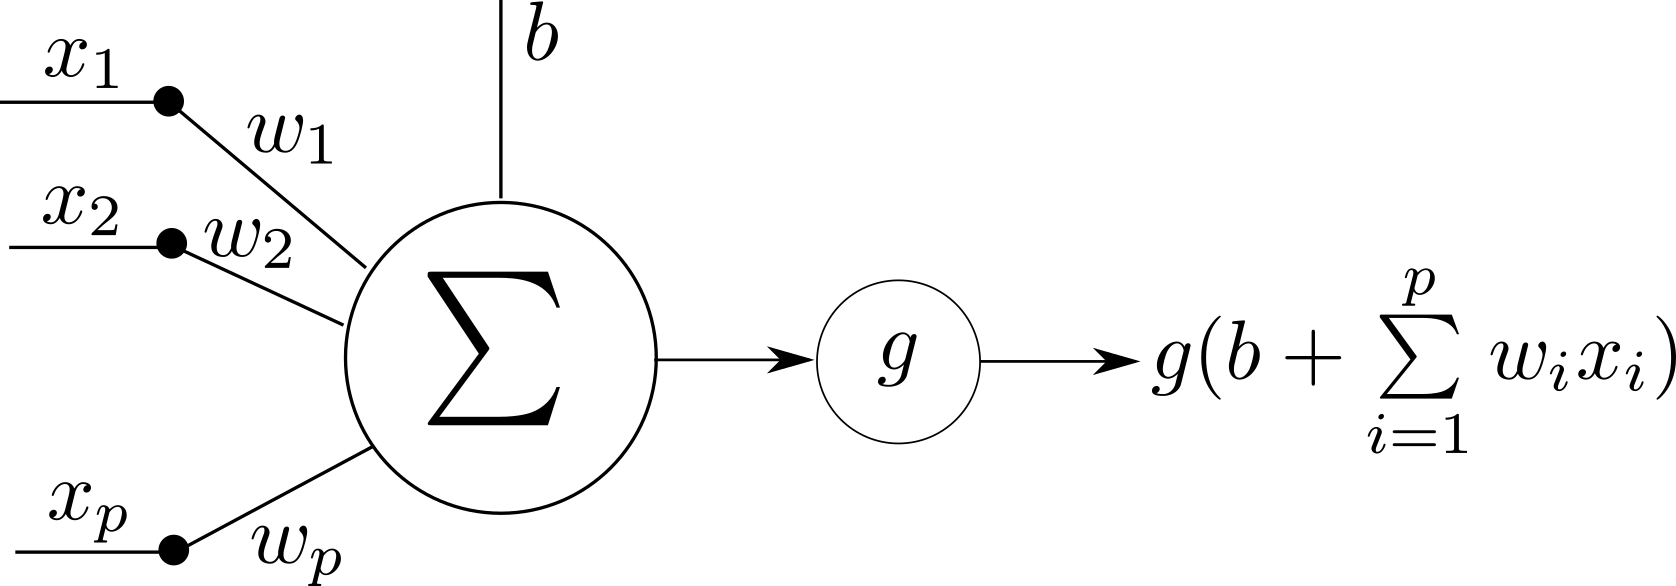
\includegraphics[height=3cm]{../graphics/neurone}
  \end{figure}

  \begin{itemize}
  \item The initial idea behind the activation function is that it works somehow as a gate
  \item If its input in ``high enough'', then the neuron is activated, i.e. a signal (other than zero) is produced
  \item It can be interpreted as a source of abstraction: information considered as unimportant is ignored
  \end{itemize}

}

%%%%%%%%%%%%%%%%%%%%%%%%%%%%%%%%%%%%%%%%%%%%%%%%%%

\frame{
  \frametitle{Activation: binary}

  \begin{columns}
    \begin{column}{.5\textwidth}
      \[
      \act(x)=
      \begin{cases}
        1,& \text{if } x > 0\\
        0,              & \text{otherwise}
      \end{cases}
      \]

    \end{column}

    \begin{column}{.5\textwidth}
      \begin{figure}
        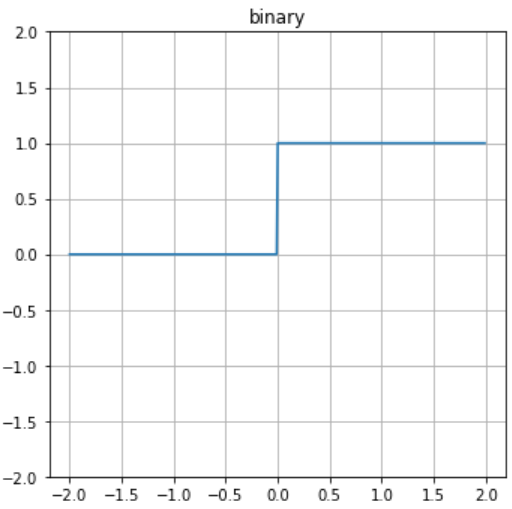
\includegraphics[width=.8\textwidth]{../graphics/act_bin.png}
      \end{figure}


    \end{column}
  \end{columns}

  \begin{block}{Remarks}
    \begin{itemize}
    \item Biologically inspired
    \item[+] Simple to compute
    \item[+] High abstraction
    \item[-] Gradient nil except on one point
    \item \alert{In practice, almost never used}
    \end{itemize}
  \end{block}


}

%%%%%%%%%%%%%%%%%%%%%%%%%%%%%%%%%%%%%%%%%%%%%%%%%%

\frame{
  \frametitle{Activation: sigmoid}

  \begin{columns}
    \begin{column}{.5\textwidth}
      \[
      \act(x)= \frac{1}{1 + e^{-x}}
      \]
    \end{column}

    \begin{column}{.5\textwidth}
      \begin{figure}
        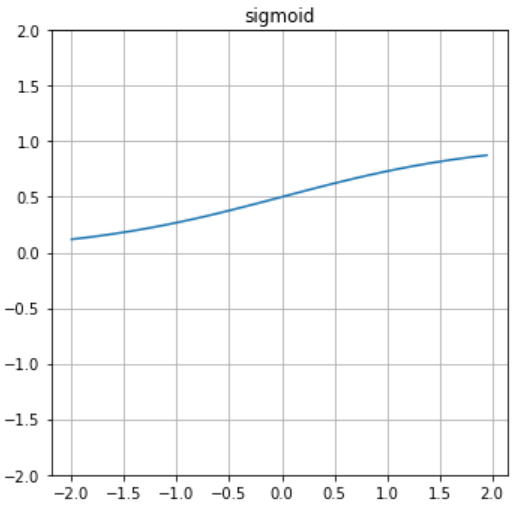
\includegraphics[width=.8\textwidth]{../graphics/act_sigm.png}
      \end{figure}


    \end{column}
  \end{columns}

  \begin{block}{Remarks}
    \begin{itemize}
    \item[+] Similar to binary activation, but with usable gradient
    \item[-] However, gradient tends to zero when input is far from zero
    \item[-] More computationally intensive
    \end{itemize}
  \end{block}



}

%%%%%%%%%%%%%%%%%%%%%%%%%%%%%%%%%%%%%%%%%%%%%%%%%%

\frame{
  \frametitle{Activation: hyperbolic tangent}

  \begin{columns}
    \begin{column}{.5\textwidth}
      \[
      \act(x)= \frac{e^x - e^{-x}}{e^x + e^{-x}}
      \]
    \end{column}

    \begin{column}{.5\textwidth}
      \begin{figure}
        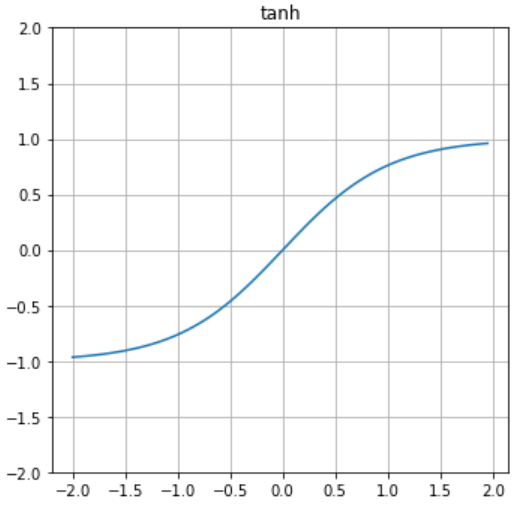
\includegraphics[width=.8\textwidth]{../graphics/act_tanh.png}
      \end{figure}


    \end{column}
  \end{columns}

  \begin{block}{Remarks}
    \begin{itemize}
    \item Similar to sigmoid
    \end{itemize}
  \end{block}



}


%%%%%%%%%%%%%%%%%%%%%%%%%%%%%%%%%%%%%%%%%%%%%%%%%%

\frame{
  \frametitle{Activation: rectified linear unit}

  \begin{columns}
    \begin{column}{.5\textwidth}
      \[
      \act(x)=
      \begin{cases}
        x,& \text{if } x > 0\\
        0,              & \text{otherwise}
      \end{cases}
      \]
    \end{column}

    \begin{column}{.5\textwidth}
      \begin{figure}
        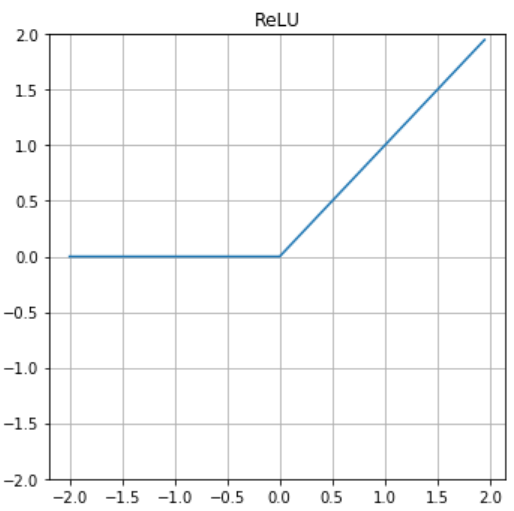
\includegraphics[width=.8\textwidth]{../graphics/act_relu.png}
      \end{figure}


    \end{column}
  \end{columns}

  \begin{block}{Remarks}
    \begin{itemize}
    \item[+] Usable gradient when activated
    \item[+] Fast to compute
    \item[+] High abstraction
    \end{itemize}
  \end{block}



}

%%%%%%%%%%%%%%%%%%%%%%%%%%%%%%%%%%%%%%%%%%%%%%%%%%
\subsection{An artificial neuron as a classifier}
%%%%%%%%%%%%%%%%%%%%%%%%%%%%%%%%%%%%%%%%%%%%%%%%%%


%%%%%%%%%%%%%%%%%%%%%%%%%%%%%%%%%%%%%%%%%%%%%%%%%%

\frame{
\frametitle{What can an artifical neuron compute?}

\begin{figure}
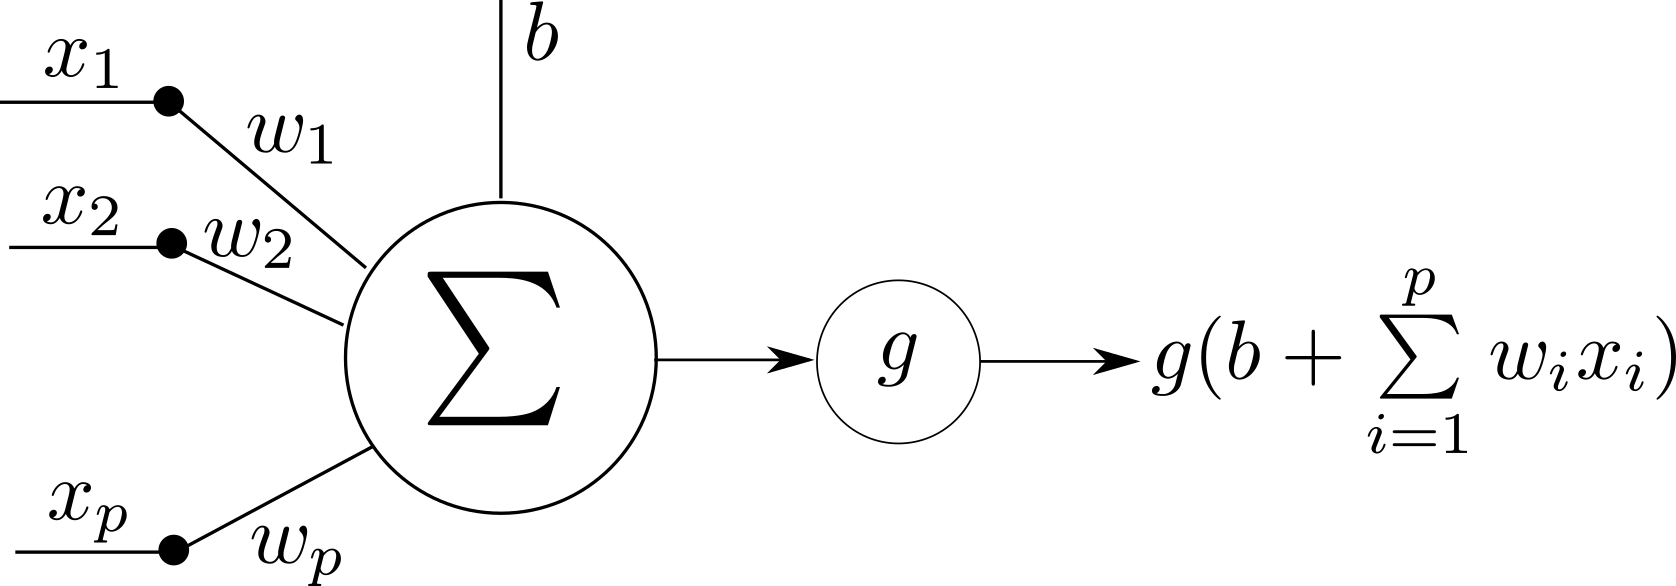
\includegraphics[height=3cm]{../graphics/neurone}
\end{figure}

\begin{block}{}
  In $\R^p$ ,
  $b + \sum\limits_{i=0}^p w_ix_i = 0$
  corresponds to a hyperplane. For a given point
  $\x = \{x_0, \ldots, x_p\}$,
  decisions are made according to the side of the hyperplane it belongs to.
\end{block}

\begin{alertblock}{}
  When the activation function is binary, we obtain a \alert{perceptron}
\end{alertblock}

}

%%%%%%%%%%%%%%%%%%%%%%%%%%%%%%%%%%%%%%%%%%%%%%%%%%

\frame{
\frametitle{Example of what we can do with a neuron}

\begin{figure}
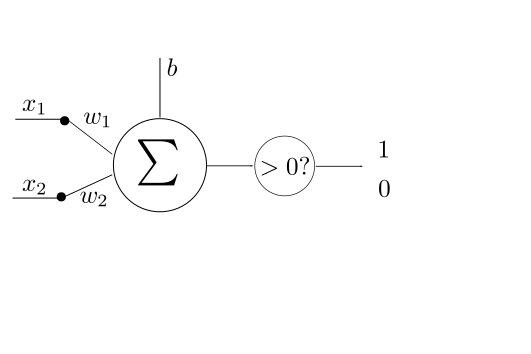
\includegraphics[height=3cm]{../graphics/neurone_simple}
\end{figure}

\begin{itemize}
\item $p=2$ : 2 dimensional inputs (can be represented on a screen!)
\item Activation: binary
\item Classification problem
\end{itemize}
}

%%%%%%%%%%%%%%%%%%%%%%%%%%%%%%%%%%%%%%%%%%%%%%%%%%

\frame{
\frametitle{Gaussian clouds}

\begin{figure}
\includegraphics[height=6cm]{../graphics/gaussian_clouds}
\end{figure}


}

%%%%%%%%%%%%%%%%%%%%%%%%%%%%%%%%%%%%%%%%%%%%%%%%%%

\frame{
\frametitle{Gaussian clouds}

\begin{figure}
\includegraphics[height=6cm]{../graphics/gaussian_clouds_H}
\end{figure}


}

%%%%%%%%%%%%%%%%%%%%%%%%%%%%%%%%%%%%%%%%%%%%%%%%%%

\frame{
\frametitle{Circles}

\begin{figure}
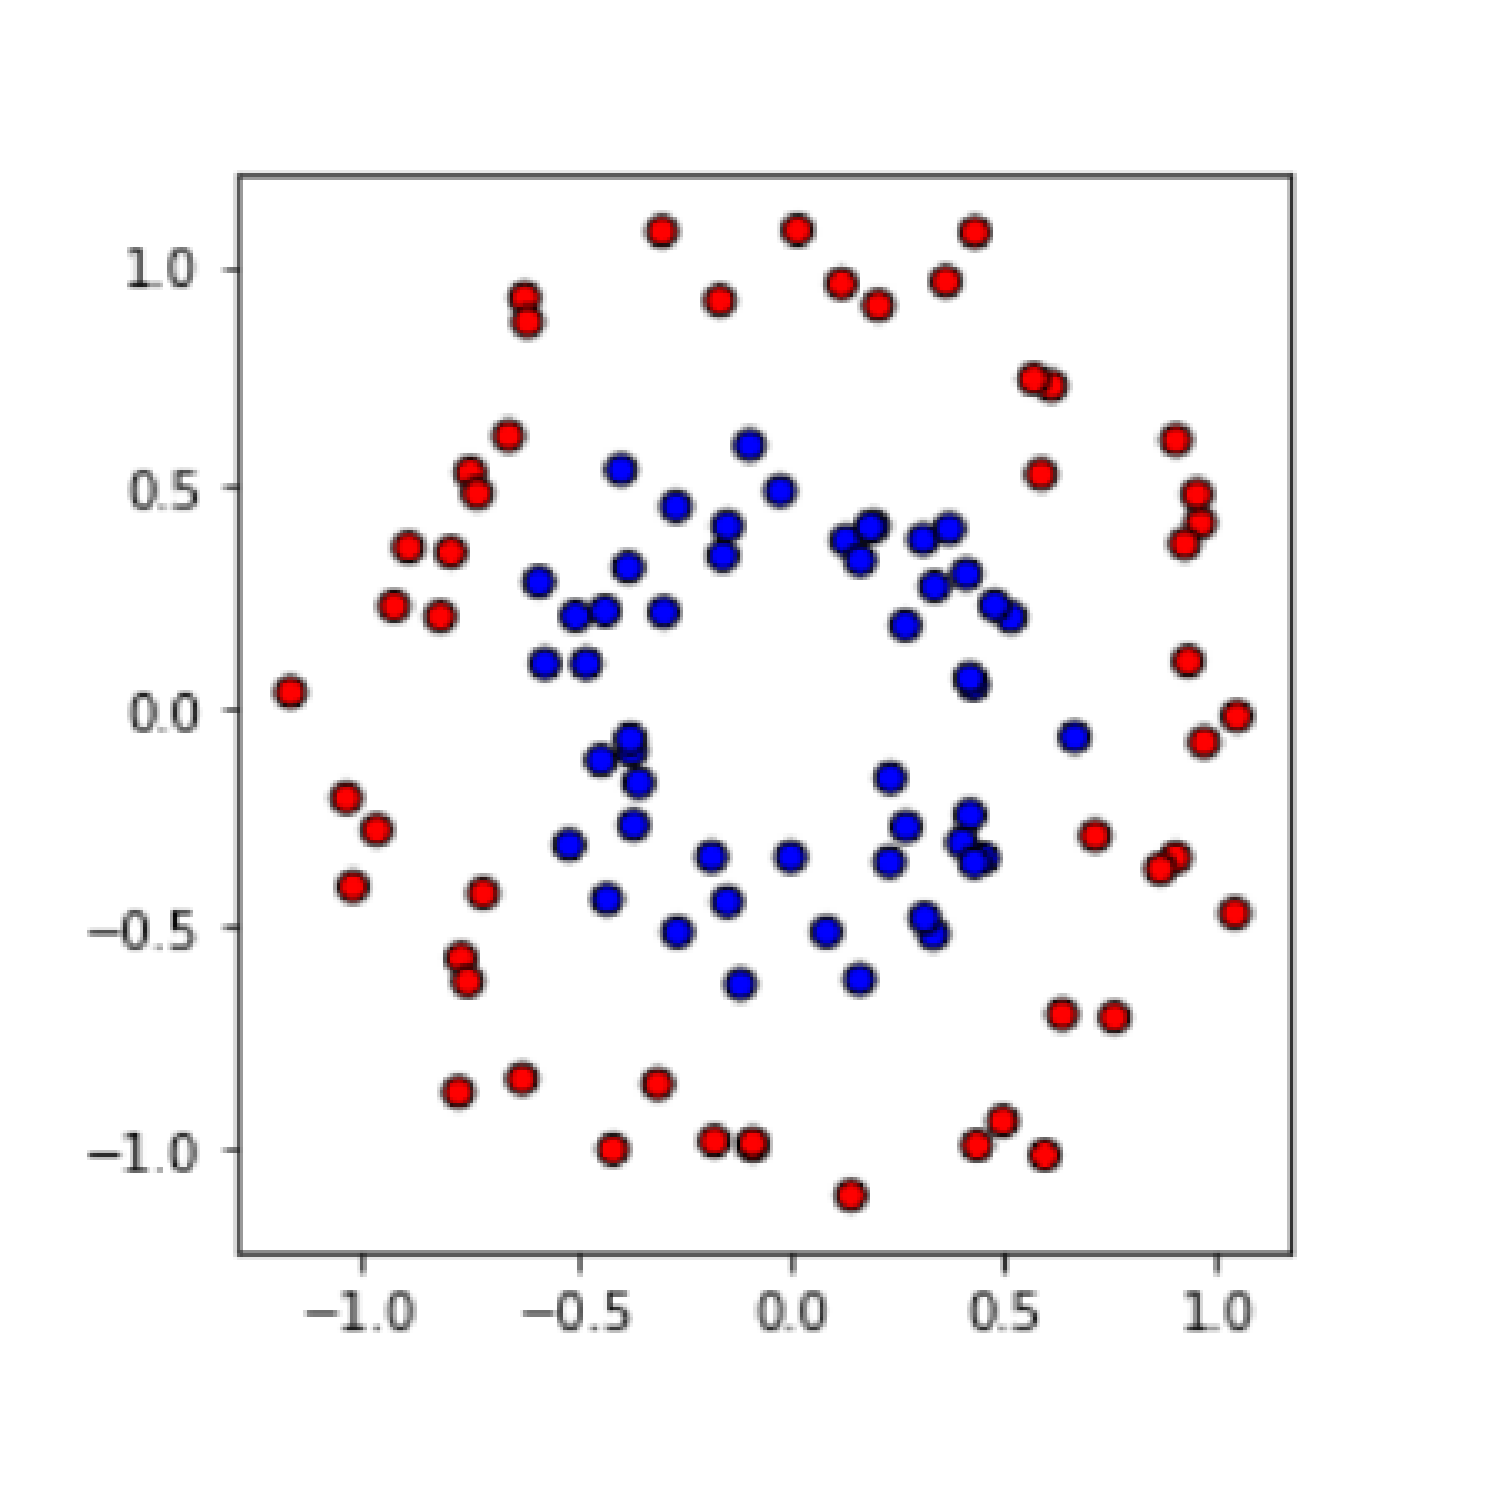
\includegraphics[height=6cm]{../graphics/circles}
\end{figure}


}

%%%%%%%%%%%%%%%%%%%%%%%%%%%%%%%%%%%%%%%%%%%%%%%%%%

\frame{
\frametitle{Circles}

\begin{figure}
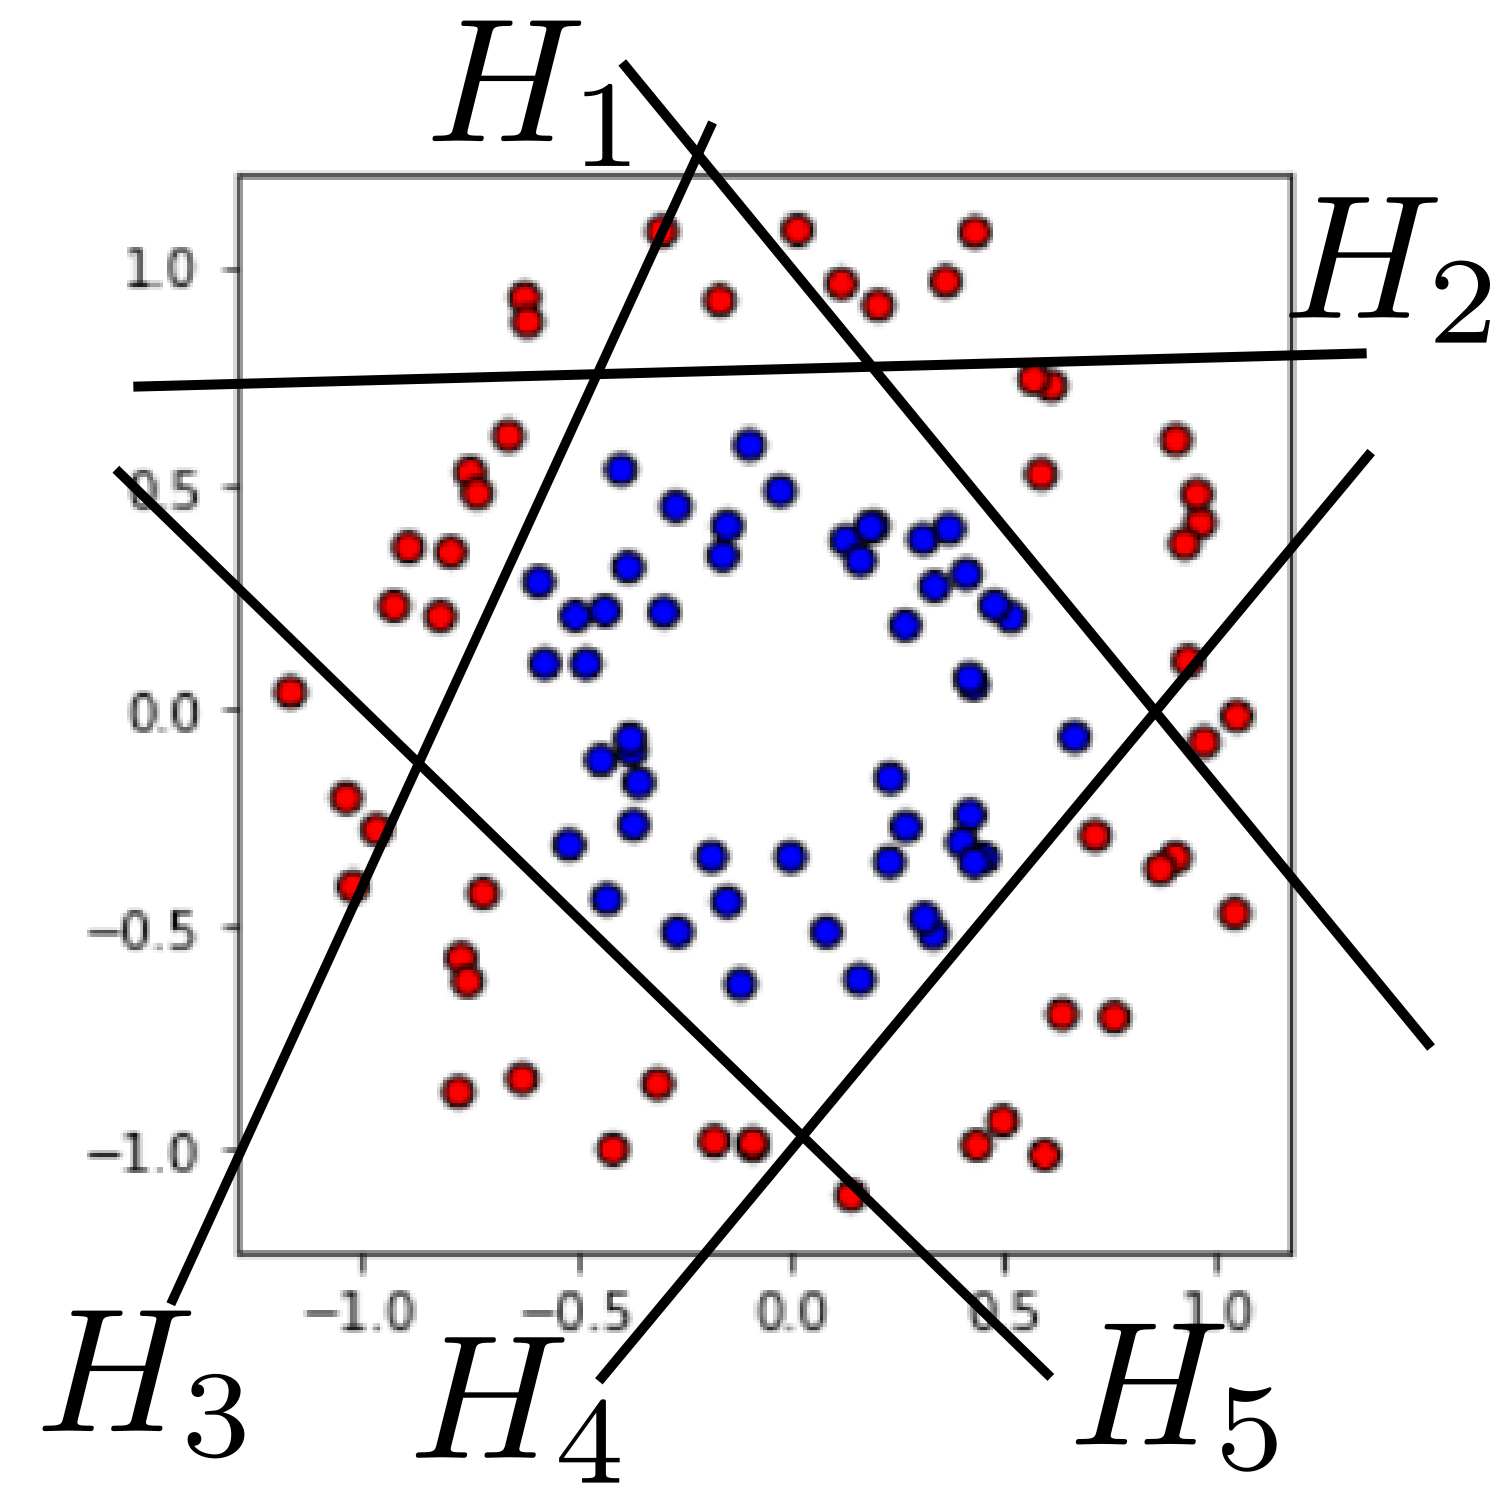
\includegraphics[height=6cm]{../graphics/circles_H}
\end{figure}

}

%%%%%%%%%%%%%%%%%%%%%%%%%%%%%%%%%%%%%%%%%%%%%%%%%%

\frame{
\frametitle{Solution}

\begin{columns}
  \begin{column}{.5\textwidth}
    \begin{figure}
      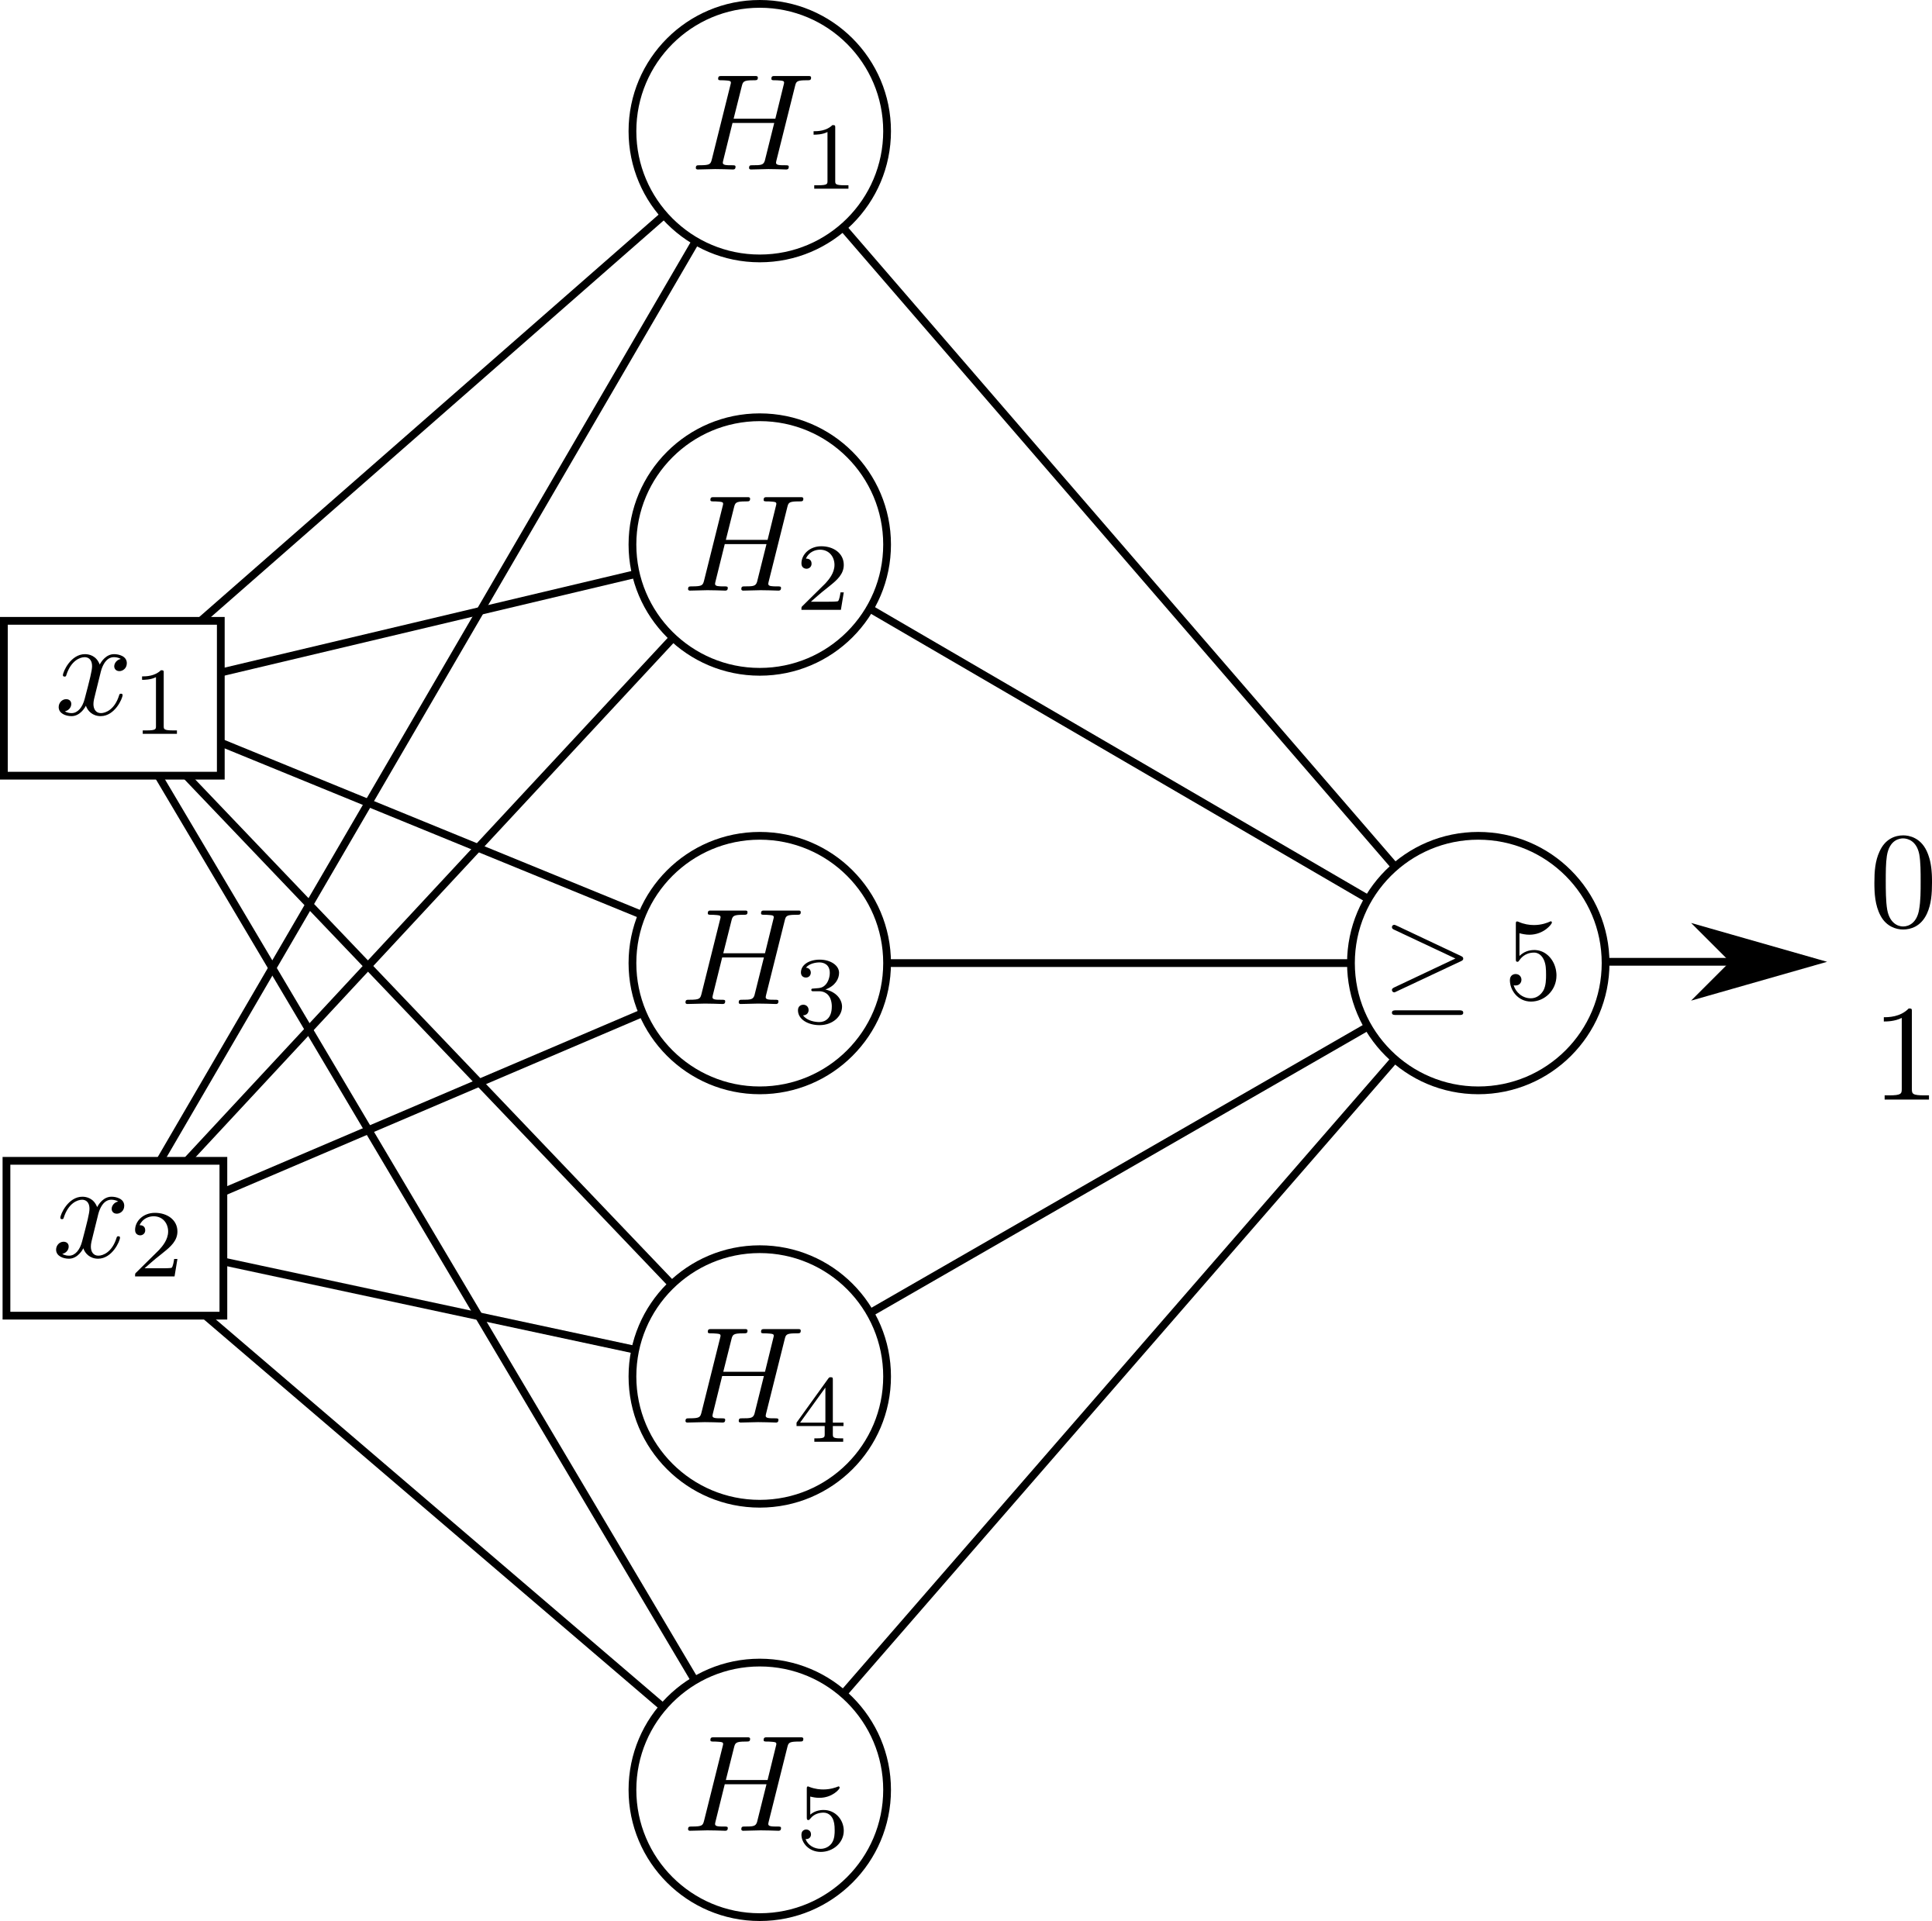
\includegraphics[height=5cm]{../graphics/ann_5}
    \end{figure}

  \end{column}

  \begin{column}{.5\textwidth}

\begin{block}{Artificial neuron compact representation}
    \begin{figure}
      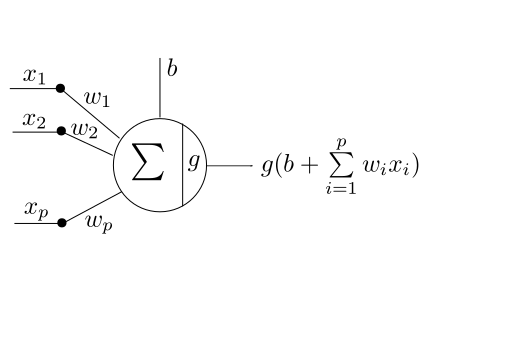
\includegraphics[height=2cm]{../graphics/neurone_representation_compacte}
    \end{figure}
\end{block}

  \end{column}
\end{columns}


}

%%%%%%%%%%%%%%%%%%%%%%%%%%%%%%%%%%%%%%%%%%%%%%%%%%
\section{Artificial neural networks}
%%%%%%%%%%%%%%%%%%%%%%%%%%%%%%%%%%%%%%%%%%%%%%%%%%

\subsection{Basic architectures}

%%%%%%%%%%%%%%%%%%%%%%%%%%%%%%%%%%%%%%%%%%%%%%
\frame{
\frametitle{Notations}

\begin{figure}
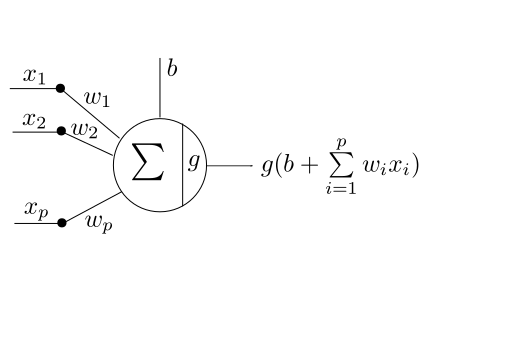
\includegraphics[height=3cm]{../graphics/neurone_representation_compacte}
\end{figure}

\begin{block}{}
  We will often use:
  \[
  \W = (w_1, \ldots, w_p)^T
  \]
  \[
  \x = (x_1, \ldots, x_p)^T
  \]
\end{block}

Therefore, we can simply write:
\[
\act(b+ \sum\limits_{i=1}^p w_ix_i) = \act(b + \W^T\x)
\]

}

%%%%%%%%%%%%%%%%%%%%%%%%%%%%%%%%%%%%%%%%%%%%%%%%%%
\frame{
\frametitle{Neural network (NN)}

\begin{block}{Definitions}
  \begin{itemize}
  \item An (artificial) neural network is a directed graph, where:
    \begin{itemize}
    \item the nodes are articial neurons and
    \item the edges are connections between the neurons.
    \end{itemize}
  \item The \alert{input layer} is the set of neurons without incoming edges.
  \item The \alert{ouput layer} is the set of neurons without outgoing edges.
  \end{itemize}


\end{block}

}


%%%%%%%%%%%%%%%%%%%%%%%%%%%%%%%%%%%%%%%%%%%%%%%%%%
\frame{
\frametitle{Feed-forward neural networks}


\begin{block}{Definition}
  \begin{itemize}
  \item A feed-forward neural networks is a NN without cycles
  \item A neuron belongs to layer $q$ if the longest path in the graph between the input layer and the neuron is of length $q$.
  \item Any layers other than input and output layers are called \alert{hidden layers}
  \end{itemize}

\end{block}

\begin{figure}
  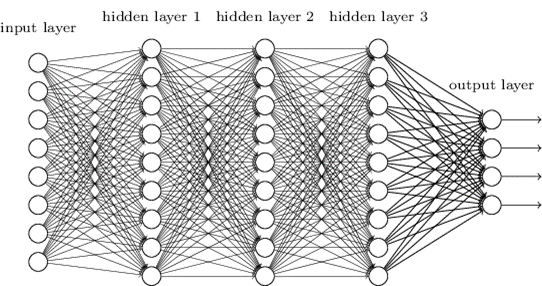
\includegraphics[height=3cm]{../graphics/network.png}
\end{figure}

{\small(from http://www.jtoy.net)}

}

%%%%%%%%%%%%%%%%%%%%%%%%%%%%%%%%%%%%%%%%%%%%%%%%%%
\frame{
\frametitle{Feed-forward neural networks}

\begin{alertblock}{}
  In the following of this course, except when otherwise specified, all NNs will be feed-forward. Indeed, this is the preferred type of NN for image processing.
\end{alertblock}

\begin{block}{What about other architectures?}
  \begin{itemize}
    \item Recurrent neural networks (RNN)
    \item Long short-term memory networks (LSTM)
  \end{itemize}
\end{block}

\begin{itemize}
  \item More powerful than feed-forward NNs
  \item More biologically realistic
  \item Complex dynamics; more difficult to train
  \item Mainly used for processing temporal data
\end{itemize}
}

%%%%%%%%%%%%%%%%%%%%%%%%%%%%%%%%%%%%%%%%%%%%%%%%%%
\frame{
\frametitle{Fully-connected network}

\begin{itemize}
\item A layer is said to be fully-connected if each of its neurons is connected to all the neurons of the previous and following layers
\item A NN is said to be fully connected if all its hidden layers are fully connected
\end{itemize}

\begin{figure}
  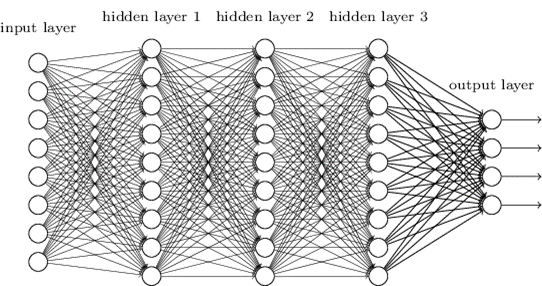
\includegraphics[height=3cm]{../graphics/network.png}
\end{figure}

}

%%%%%%%%%%%%%%%%%%%%%%%%%%%%%%%%%%%%%%%%%%%%%%%%%%
\frame{
\frametitle{Number of parameters}

\begin{figure}
  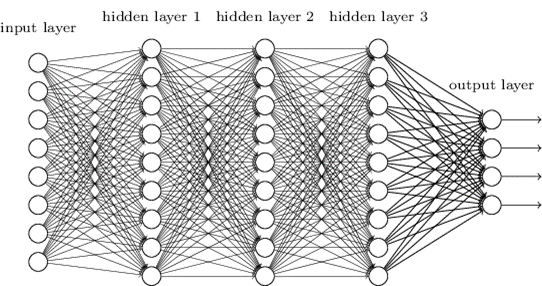
\includegraphics[height=3cm]{../graphics/network.png}
\end{figure}

\begin{itemize}
\item How many parameters does the above network contain?
\item<2-> First hidden layer:
\item<3-> $9$ neurons $\times 8$ neurons in the previous layer $+ 9$ biases $=81$
\item<4-> Second and third layers: $9 \times 9 + 9 =90$
\item<5-> Output layer: $4 \times 9 + 4$
\item<6-> Total: $305$ parameters
\end{itemize}

}

%%%%%%%%%%%%%%%%%%%%%%%%%%%%%%%%%%%%%%%%%%%%%%%%%%
\subsection{The power of neural networks}


%%%%%%%%%%%%%%%%%%%%%%%%%%%%%%%%%%%%%%%%%%%%%%%%%%
\frame{
\frametitle{Universal approximation theorem}

\begin{columns}
  \begin{column}{.5\textwidth}
    \begin{itemize}
    \item We have previously seen that a neuron can be used as a linear classifier and that combining several of them one can build complex classifiers
    \item We will see that this observation can be generalized
    \end{itemize}
  \end{column}

  \begin{column}{.5\textwidth}
    \begin{figure}
      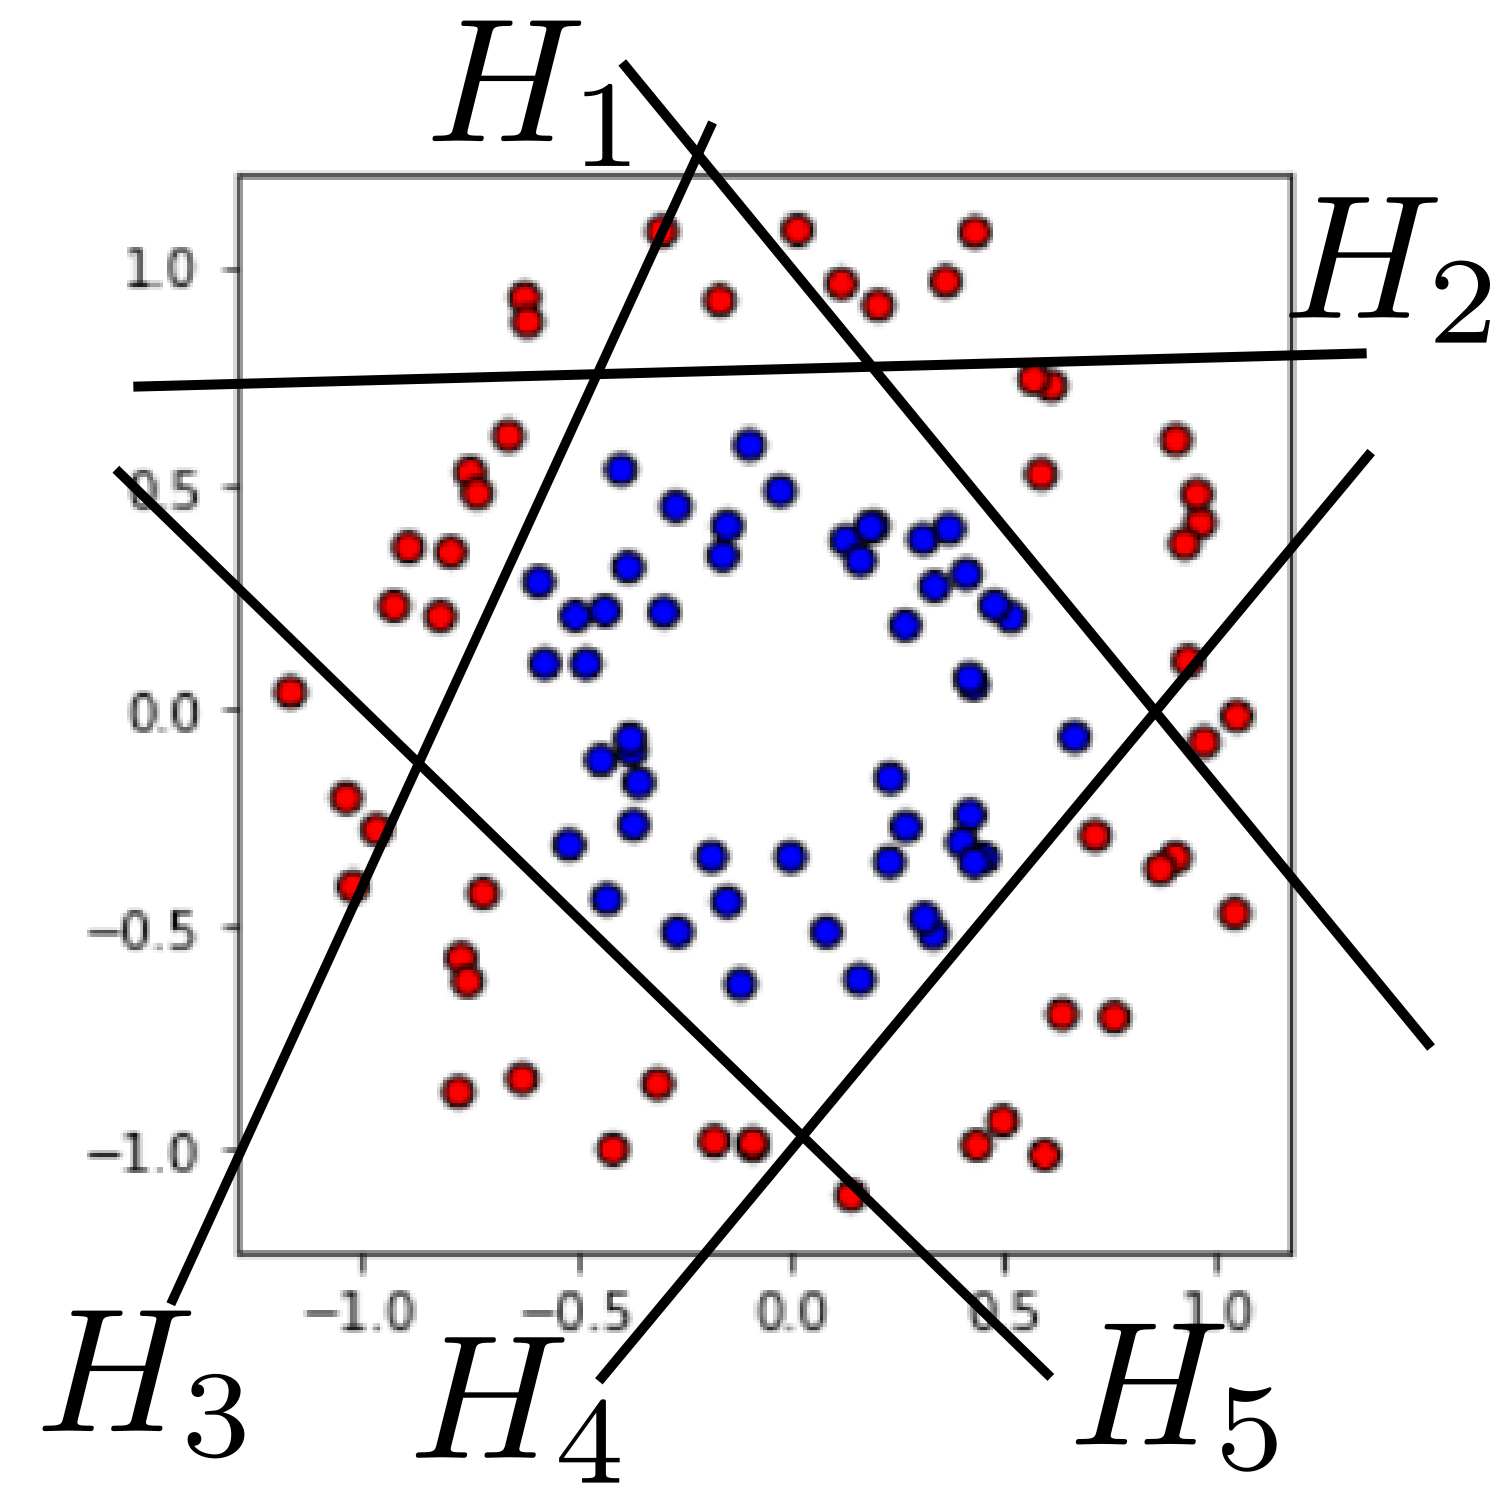
\includegraphics[height=4cm]{../graphics/circles_H}
    \end{figure}
  \end{column}
\end{columns}


}

%%%%%%%%%%%%%%%%%%%%%%%%%%%%%%%%%%%%%%%%%%%%%%%%%%
\frame{
\frametitle{Universal approximation theorem}

\begin{block}{}
  Let $f$ be a \textcolor{blue}{continuous} real-valued function of $[0,1]^p$ ($p \in \N^*$) and $\epsilon$ a strictly positive real. Let $\act$ be a non-constant, increasing, bounded real function (\emph{\small{the activation function}}).

  Then there exist an integer $n$, real vectors $\{\W_i\}_{1 \leq n}$ of $\R^p$, and reals $\{b_i\}_{1 \leq n}$ and $\{v_i\}_{1 \leq n}$ such that for all $\x$ in $[0,1]^p$:

  \[
   \left| f(\x) - \sum\limits_{i=1}^n v_i \act(\W_i^T\x + b_i) \right| < \epsilon
  \]

\end{block}

A first version of this theorem, using sigmoidal activation functions, was proposed by \cite{cybenko_approximations_1989}. The version above was demonstrated by \cite{hornik_approximation_1991}.

}

%%%%%%%%%%%%%%%%%%%%%%%%%%%%%%%%%%%%%%%%%%%%%%%%%%
\frame{
\frametitle{Universal approximation theorem: what does it mean?}

  \[
   \left| f(\x) - \sum\limits_{i=1}^n v_i \act(\W_i^T\x + b_i) \right| < \epsilon
  \]

This means that function $f$ can be approximated with a neural network containing:
\begin{itemize}
  \item an input layer of size $p$;
  \item a hidden layer containing $n$ neurons with activation function $\act$, weights $\W_i$ and biases $b_i$;
  \item an output layer containing a single neuron, with weigths $v_i$ (and an identity activation function).
\end{itemize}

}


%%%%%%%%%%%%%%%%%%%%%%%%%%%%%%%%%%%%%%%%%%%%%%%%%%
\frame{
  \frametitle{Universal approximation theorem in practice}

  \begin{itemize}
  \item The number of neurons increases very rapidly with the complexity of the function
  \item Empirical evidence has shown that multi-layer architectures give better results
  \end{itemize}

  \begin{block}<2->{}
    A NN can potentially have a lot of parameters. How can we set them?
\end{block}

}



%%%%%%%%%%%%%%%%%%%%%%%%%%%%%%%%%%%%%%%%%%%%%%%%%
\section{Training a neural network}
%%%%%%%%%%%%%%%%%%%%%%%%%%%%%%%%%%%%%%%%%%%%%%%%%

%%%%%%%%%%%%%%%%%%%%%%%%%%%%%%%%%%%%%%%%%%%%%%%%%
\begin{frame}{Introduction}

\begin{itemize}
\item We have seen that NNs have a lot of potential. However, how can the parameters $\param = (\W_i, \bias_i)$  be set?
\item What is our objective ?
\item A very general solution, that is also the mostly used, is \alert{gradient descent}
\end{itemize}

\end{frame}


%%%%%%%%%%%%%%%%%%%%%%%%%%%%%%%%%%%%
\begin{frame}{Learning problem}

  We recall that our training set contains $n$ samples:

  \[
  (\x_i, y_i) \in \R^p \times \R
  \]

  We \textcolor{blue}{choose} a family $f_{\param}$
  of functions from $\R^p$ into $\R$,
  depending on our set of parameters $\param$,
  and \textcolor{blue}{find} the value of $\param$
  that minimizes a \textcolor{blue}{chosen} loss function $\loss$:

\[
\param ^{\ast} = \argmin_{\param} ( \loss (\param) + \mathcal{R}(\param) )
\]

where $\mathcal{R}(\param)$ is a regularization term.

\vspace{1em}

\small{For the time being, for the sake of simplicity, we will drop the regularization term until further notice}

\end{frame}

%%%%%%%%%%%%%%%%%%%%%%%%%%%%%%%%%%%%
\begin{frame}{Loss function}

  A general form of the loss function is:
  \[
  \loss(\param) = \sum\limits_{i=1}^n d(y_i, f(\x_i, \theta))
  \]
  where $d$ is some disparity function (the more similar its parameters, the smaller its value).

\end{frame}


%%%%%%%%%%%%%%%%%%%%%%%%%%%%%%%%%%%%
\begin{frame}{Loss function: examples}


  \begin{block}{Squared error}
    \[
    \loss(\param) = \sum\limits_{i=1}^n (y_i - f(\x_i, \theta))^2
    \]
    This loss function is mainly used in regression problems. However, it has also been used for binary classification problems.
  \end{block}

  \begin{block}{Cross-entropy}
    In this case, $\x_i \in \{0, 1\}^p$ and $y_i \in [0, 1]$:
    \[
    \loss(\param) = \sum\limits_{i=1}^n y_i ln( f(\x_i, \theta) )
    \]
    This loss function is used in binary classification problems, where the network's output can be interpreted as a probability of belonging to a class.
  \end{block}

\end{frame}


%%%%%%%%%%%%%%%%%%%%%%%%%%%%%%%%%%%%
\begin{frame}{Gradient descent}

\begin{block}{Definition}
  Gradient descent is an optimization algorithm. For a derivable function $\loss$, a positive real $\gamma$ (the \alert{learning rate}) and a starting point $\param_0$, it computes a sequence of values:
  \[
  \forall i \in \N: \param_{i+1} = \param_i - \gamma \nabla \loss(\param_i)
  \]
\end{block}

\begin{block}{Property}
  If $\gamma$ is small enough, then:
  \[
  \loss(\param_{i+1}) \leq \loss(\param_i)
  \]
\end{block}

Gradient descent is an essential tool in optimization.

\end{frame}

%%%%%%%%%%%%%%%%%%%%%%%%%%%%%%%%%%%%
\begin{frame}{Gradient descent in the scalar case}

\begin{columns}
  \begin{column}{.5\textwidth}
    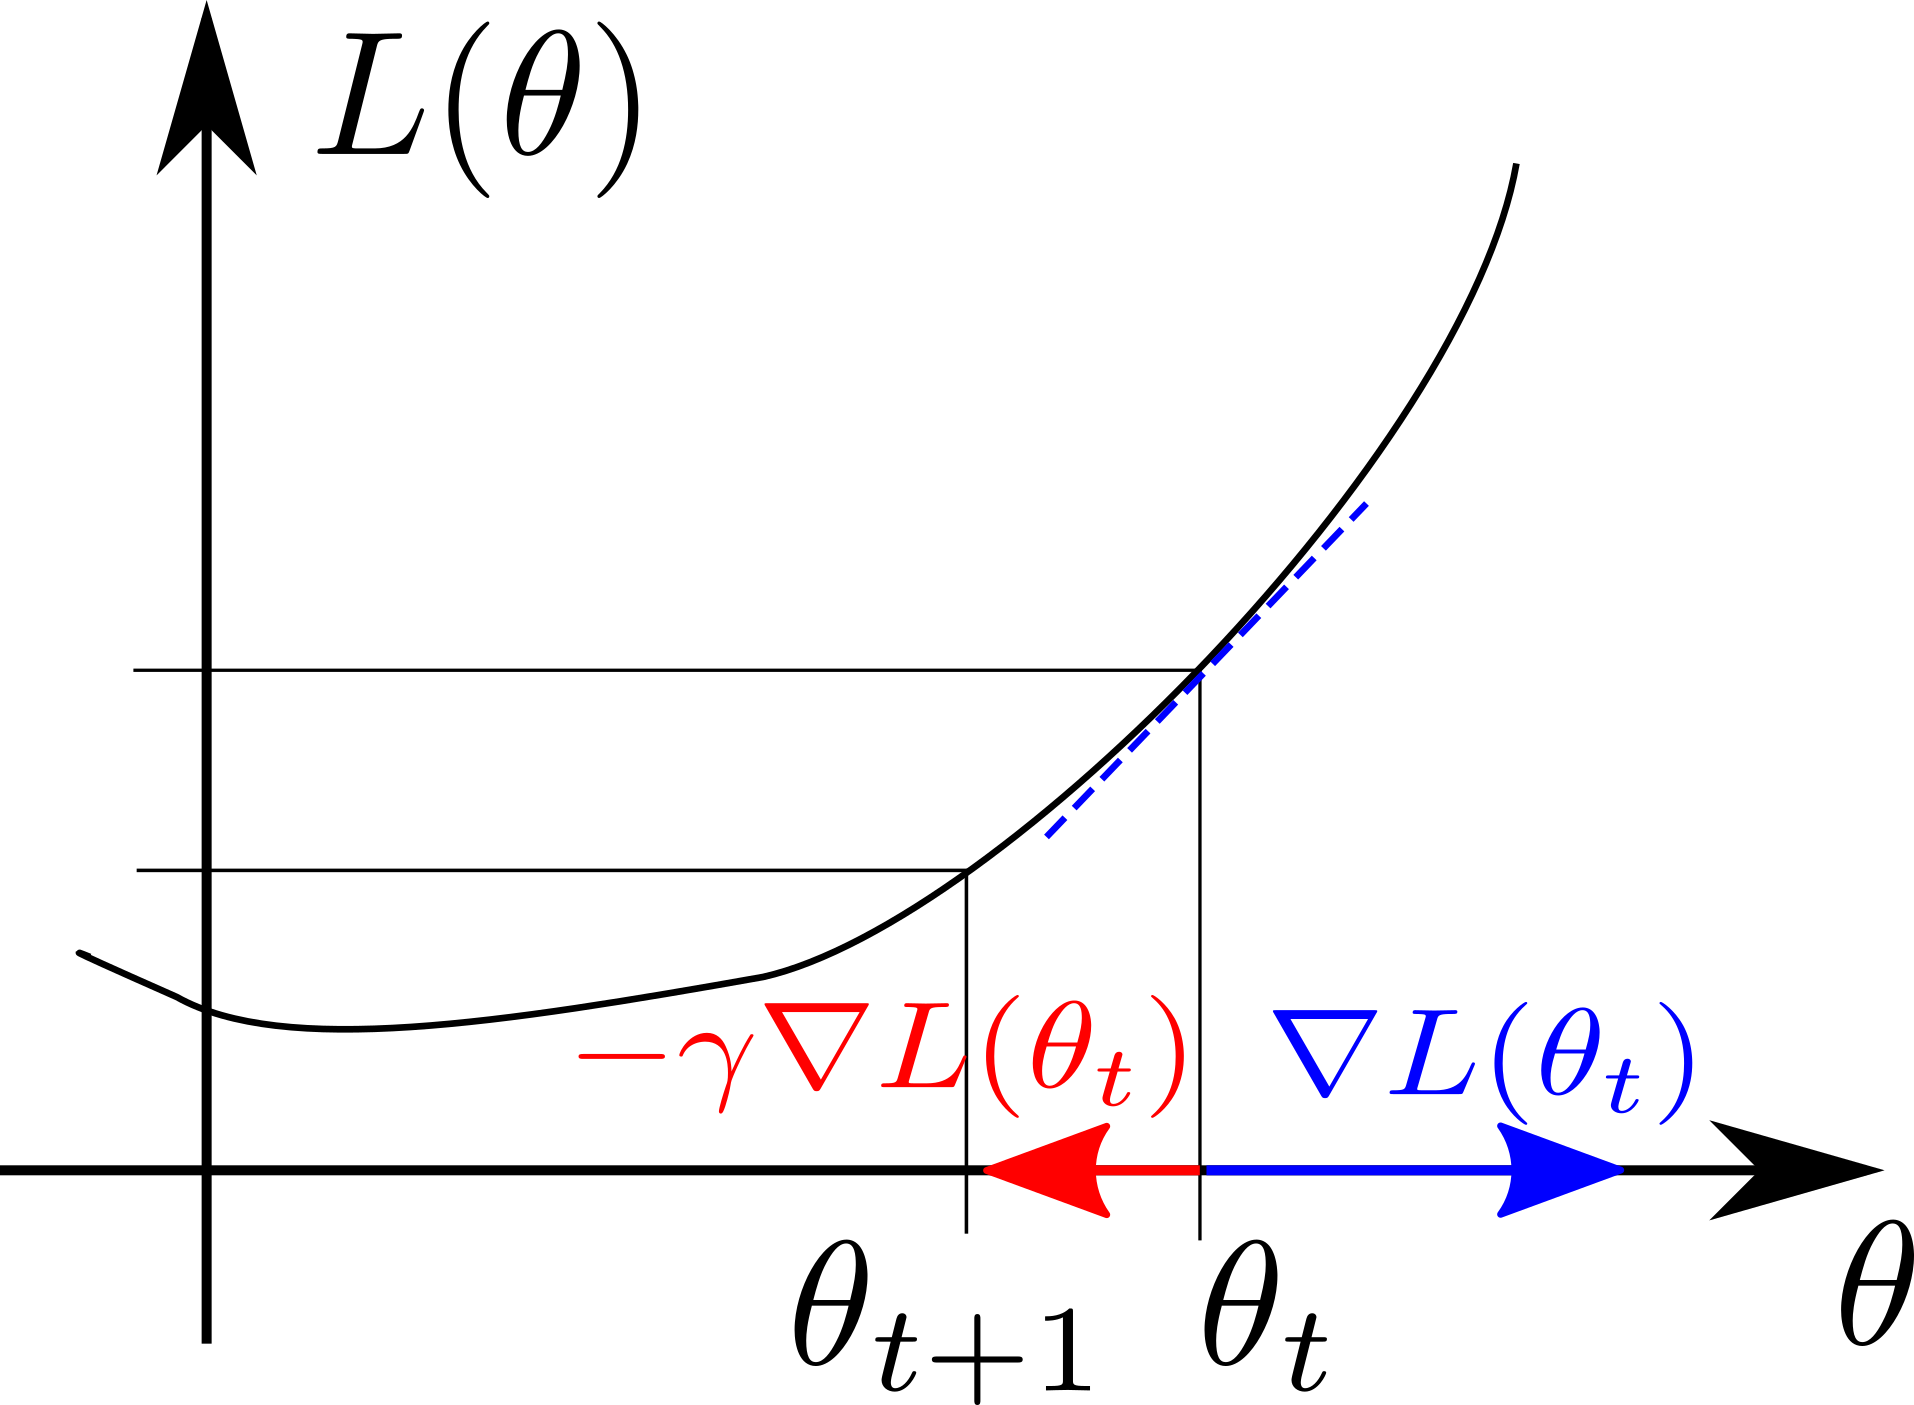
\includegraphics[width=\textwidth]{../graphics/gradient_descent}
  \end{column}

  \begin{column}{.5\textwidth}
    \[
    \theta_{t+1} = \theta_t - \gamma\nabla \loss(\theta_t)
    \]
  \end{column}
\end{columns}

\end{frame}


%%%%%%%%%%%%%%%%%%%%%%%%%%%%%%%%%%%%
\begin{frame}{Gradient descent applied to neural networks}

  In the case of neural networks, the loss $\loss$ depends on each parameter $\theta_i$ via the composition of several simple functions. In order to compute the gradient $\nabla_{\param}\loss$ we will make extensive use of the chain rule theorem.

  \begin{block}{Chain rule theorem}
    Let $f_1$ and $f_2$ be two derivable real functions ($\R \rightarrow \R$). Then for all $x$ in $\R$:   :
    \[
     (f_2 \circ f_1)'(x) = f_2'(f_1(x)).f_1'(x)
    \]
  \end{block}


\begin{block}{Leibniz notation}
  Let us introduce variables, $x$, $y$ and $z$:
  \[x \xrightarrow{f_1} y \xrightarrow{f_2} z\]

  Then:
  \[\dv{z}{x} = \dv{z}{y} \cdot \dv{y}{x} \]

\end{block}

\end{frame}















%%%%%%%%%%%%%%%%%%%%%%%%%%%%%%%%%%%%%%%%%%%%%%%%%
\begin{frame}{Backpropagation through a fully connected layer}
\begin{figure}
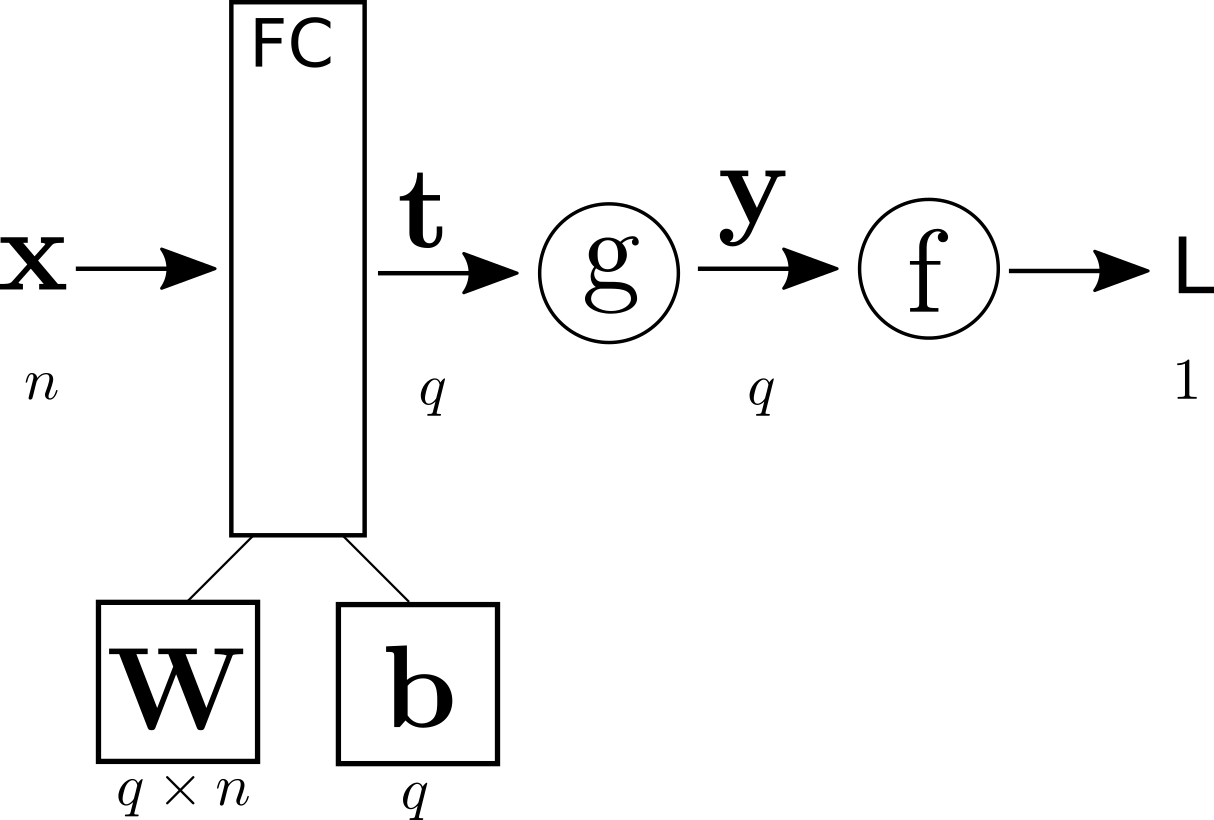
\includegraphics[width=0.5\textwidth]{../graphics/bp_fc.png}
\end{figure}

Setup:
\begin{eqnarray*}
n, q \in \N^*\\
\x \in \R^n \\
\W \in \R^q \times \R^n \\
\bias, \mathbf{t}, \y \in \R^q \\
\loss \in \R
\end{eqnarray*}

\end{frame}

%%%%%%%%%%%%%
\begin{frame}{Backpropagation through a fully connected layer}
\begin{figure}
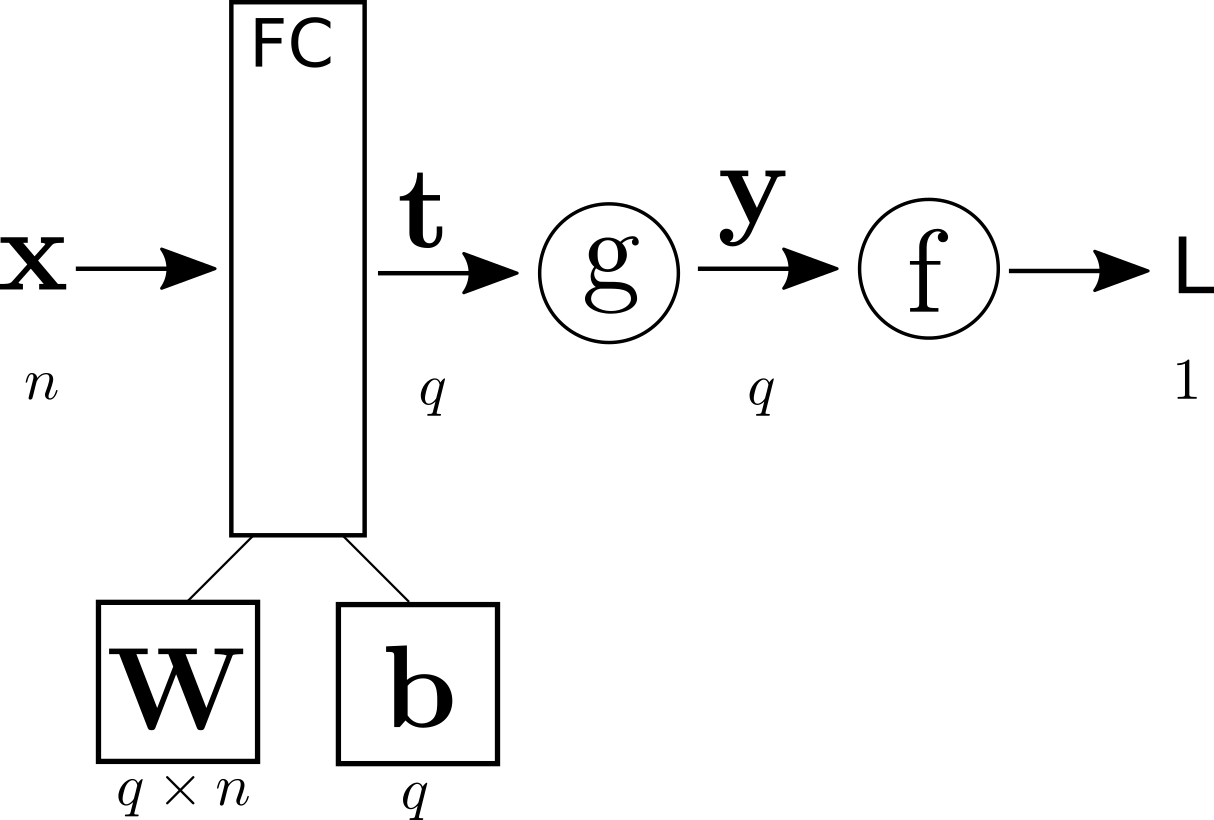
\includegraphics[width=0.5\textwidth]{../graphics/bp_fc.png}
\end{figure}

\begin{columns}
  \begin{column}{0.5\textwidth}
    Forward pass:
    \begin{eqnarray*}
      \mathbf{t} &=& \W\x + \bias \\
      \y &=& \act(\W\x + \bias) \\
      \loss &=& \loss(\y)
    \end{eqnarray*}
  \end{column}

  \begin{column}{0.5\textwidth}
    Local gradients:
    \begin{eqnarray*}
      \pdv{\mathbf{t}}{\W} &=& \x^t \\
      \pdv{\mathbf{t}}{\bias} &=& 1 \\
      \pdv{\y}{\mathbf{t}} &=& \act'
    \end{eqnarray*}
  \end{column}
\end{columns}

\end{frame}

%%%%%%%%%%%%%
\begin{frame}{Backpropagation through a fully connected layer}
  \begin{figure}
    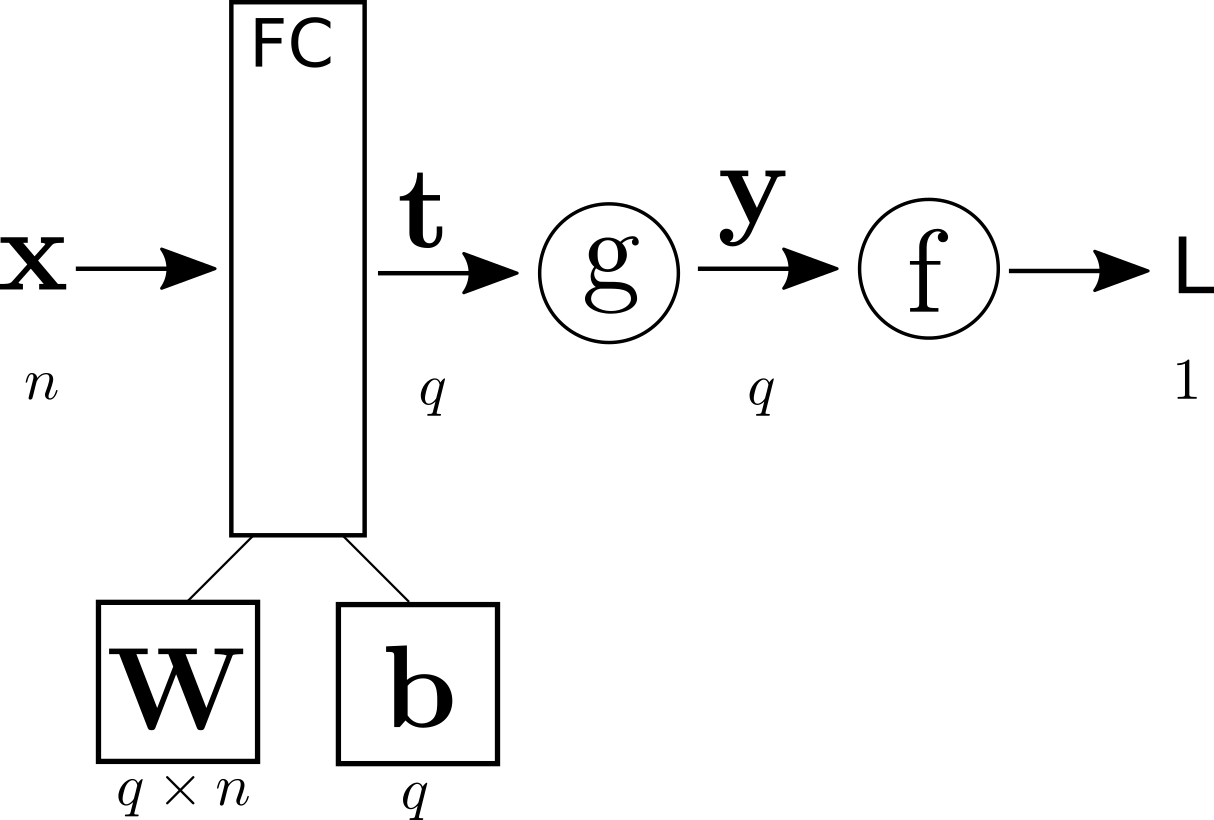
\includegraphics[width=0.5\textwidth]{../graphics/bp_fc.png}
  \end{figure}

  Backpropagation:
  \begin{eqnarray*}
    \pdv{\loss}{\mathbf{t}} &=& \pdv{\loss}{\y}.\pdv{\y}{\mathbf{t}} \\
                           &=& \pdv{\loss}{\y} \odot \act'(\mathbf{t}) \\
  \end{eqnarray*}

\end{frame}

%%%%%%%%%%%%%
\begin{frame}{Backpropagation through a fully connected layer}
  \begin{figure}
    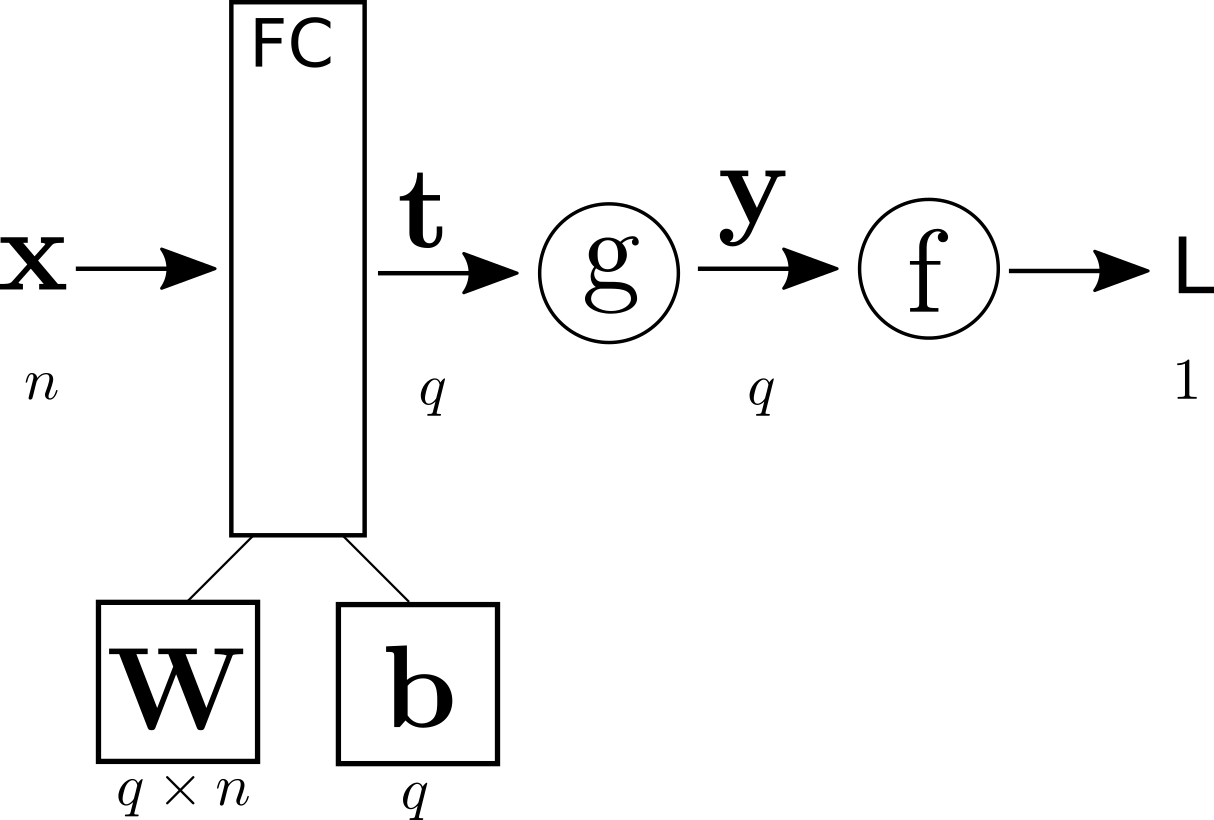
\includegraphics[width=0.5\textwidth]{../graphics/bp_fc.png}
  \end{figure}

  Backpropagation:
  \begin{columns}
    \begin{column}{.5\textwidth}
      \begin{eqnarray*}
        \pdv{\loss}{\W} &=& \pdv{\loss}{\mathbf{t}}.\pdv{\mathbf{t}}{\W} \\
                   &=& \pdv{\loss}{\y} \odot \act'(\mathbf{t}).\x^t
      \end{eqnarray*}
    \end{column}

  \begin{column}{.5\textwidth}
  \begin{eqnarray*}
    \pdv{\loss}{\bias} &=&  \pdv{\loss}{\y} \odot \act'(\mathbf{t})
  \end{eqnarray*}
  \end{column}
\end{columns}


\end{frame}

%%%%%%%%%%%%%%%%%%%%%%%%%%%%%%%%%%%%%%%%%%%%%%%%%
\section{Deep learning today and tomorrow}


%%%%%%%%%%%%%%%%%%%%%%%%%%%%%%%%%%%%%%%%%%%%%%%%%%

\frame{
\frametitle{The triggering factor to the success of neural networks}

\begin{itemize}

\item Appropriate architectures: graphical processing units (GPUs)
\item Optimized software
\item Large annotated databases

\end{itemize}

}

%%%%%%%%%%%%%%%%%%%%%%%%%%%%%%%%%%%%%%%%%%%%%%%%%%

\frame{
\frametitle{Practical considerations}

For a deep-learning solution to work, you need:

\begin{itemize}

\item A lot of annotated data
\item A lot of fiddling (different architectures; hyper-parameters)
\item GPUs, at least from training

\end{itemize}

Deep learning can produce astonishing results \cite{nguyen_deep_2015}...
\begin{figure}
  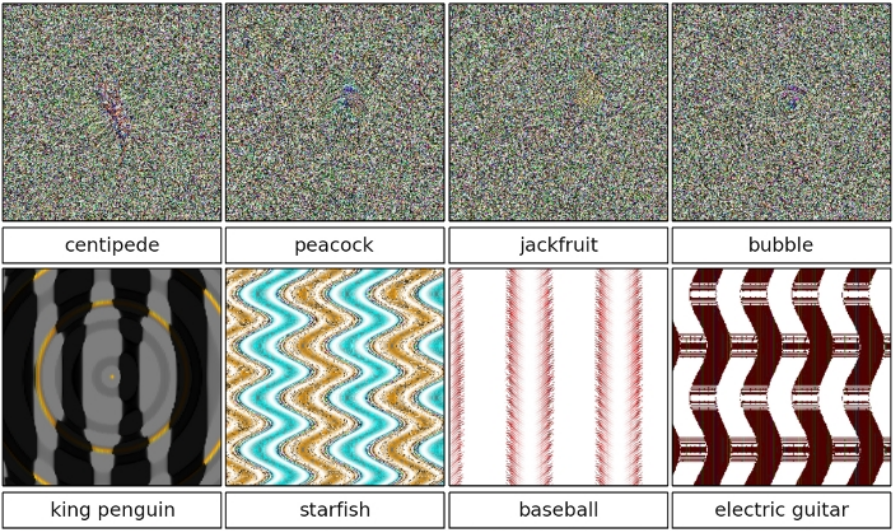
\includegraphics[height=3cm]{../graphics/dl_easily_fooled.png}
\end{figure}


}


%%%%%%%%%%%%%%%%%%%%%%%%%%%%%%%%%%%%%%%%%%%%%%%%%%

\frame{
\frametitle{The web giants}

\begin{itemize}

\item Google, Facebook, Microsoft, Amazon etc. are actively investing in deep-learning
  \item Competition is intense
  \item Most of them are sharing their deep learning libraries

\end{itemize}

}




%%%%%%%%%%%%%%%%%%%%%%%%%%%%%%%%%%%%%%%%%%%%%%%%%%
\section*{References}

%%%%%%%%%%%%%%%%%%%%%%%%%%%%%%%%%%%%%%%%%%%%%%%%%%

\frame[allowframebreaks]{

\scriptsize

\frametitle{References}

%\bibliographystyle{amsalpha}
%\bibliographystyle{apalike}

\bibliography{edf.bib}

\normalsize

}

%%%%%%%%%%%%%%%%%%%%%%%%%%%%%%%%%%%%%%%%%%%%%%%%%%
%%%%%%%%%%%%%%%%%%%%%%%%%%%%%%%%%%%%%%%%%%%%%%%%%%
%%%%%%%%%%%%%%%%%%%%%%%%%%%%%%%%%%%%%%%%%%%%%%%%%%

\end{document}
